% Options for packages loaded elsewhere
\PassOptionsToPackage{unicode}{hyperref}
\PassOptionsToPackage{hyphens}{url}
%
\documentclass[
  11pt,
]{article}
\usepackage{lmodern}
\usepackage{amssymb,amsmath}
\usepackage{ifxetex,ifluatex}
\ifnum 0\ifxetex 1\fi\ifluatex 1\fi=0 % if pdftex
  \usepackage[T1]{fontenc}
  \usepackage[utf8]{inputenc}
  \usepackage{textcomp} % provide euro and other symbols
\else % if luatex or xetex
  \usepackage{unicode-math}
  \defaultfontfeatures{Scale=MatchLowercase}
  \defaultfontfeatures[\rmfamily]{Ligatures=TeX,Scale=1}
\fi
% Use upquote if available, for straight quotes in verbatim environments
\IfFileExists{upquote.sty}{\usepackage{upquote}}{}
\IfFileExists{microtype.sty}{% use microtype if available
  \usepackage[]{microtype}
  \UseMicrotypeSet[protrusion]{basicmath} % disable protrusion for tt fonts
}{}
\makeatletter
\@ifundefined{KOMAClassName}{% if non-KOMA class
  \IfFileExists{parskip.sty}{%
    \usepackage{parskip}
  }{% else
    \setlength{\parindent}{0pt}
    \setlength{\parskip}{6pt plus 2pt minus 1pt}}
}{% if KOMA class
  \KOMAoptions{parskip=half}}
\makeatother
\usepackage{xcolor}
\IfFileExists{xurl.sty}{\usepackage{xurl}}{} % add URL line breaks if available
\IfFileExists{bookmark.sty}{\usepackage{bookmark}}{\usepackage{hyperref}}
\hypersetup{
  pdftitle={10. Assessment of the Northern Rockfish stock in the Gulf of Alaska},
  pdfauthor={Benjamin C. Williams, Peter-John F. Hulson, Chris R. Lunsford, Curry J. Cunningham, Dana H. Hanselman},
  hidelinks,
  pdfcreator={LaTeX via pandoc}}
\urlstyle{same} % disable monospaced font for URLs
\usepackage[top=1in,bottom=1in,left=1in,right=1in]{geometry}
\usepackage{longtable,booktabs}
% Correct order of tables after \paragraph or \subparagraph
\usepackage{etoolbox}
\makeatletter
\patchcmd\longtable{\par}{\if@noskipsec\mbox{}\fi\par}{}{}
\makeatother
% Allow footnotes in longtable head/foot
\IfFileExists{footnotehyper.sty}{\usepackage{footnotehyper}}{\usepackage{footnote}}
\makesavenoteenv{longtable}
\usepackage{graphicx,grffile}
\makeatletter
\def\maxwidth{\ifdim\Gin@nat@width>\linewidth\linewidth\else\Gin@nat@width\fi}
\def\maxheight{\ifdim\Gin@nat@height>\textheight\textheight\else\Gin@nat@height\fi}
\makeatother
% Scale images if necessary, so that they will not overflow the page
% margins by default, and it is still possible to overwrite the defaults
% using explicit options in \includegraphics[width, height, ...]{}
\setkeys{Gin}{width=\maxwidth,height=\maxheight,keepaspectratio}
% Set default figure placement to htbp
\makeatletter
\def\fps@figure{htbp}
\makeatother
\setlength{\emergencystretch}{3em} % prevent overfull lines
\providecommand{\tightlist}{%
  \setlength{\itemsep}{0pt}\setlength{\parskip}{0pt}}
\setcounter{secnumdepth}{-\maxdimen} % remove section numbering
\usepackage{booktabs}
\usepackage{longtable}
\usepackage{array}
\usepackage{multirow}
\usepackage{wrapfig}
\usepackage{float}
\usepackage{colortbl}
\usepackage{pdflscape}
\usepackage{tabu}
\usepackage{threeparttable}
\usepackage{threeparttablex}
\usepackage[normalem]{ulem}
\usepackage{makecell}
\usepackage{xcolor}

\title{10. Assessment of the Northern Rockfish stock in the Gulf of Alaska}
\author{Benjamin C. Williams, Peter-John F. Hulson, Chris R. Lunsford, Curry J. Cunningham, Dana H. Hanselman}
\date{September 2020}

\begin{document}
\maketitle

\pagenumbering{gobble}

\hypertarget{references}{%
\section*{References}\label{references}}
\addcontentsline{toc}{section}{References}

\hypertarget{refs}{}

\pagebreak

\hypertarget{tables}{%
\section{Tables}\label{tables}}

\begin{tabular}{l|r|r|r|r|r|r|r|r|r|r|r|r|r|r|r}
\hline
name & X1991 & X1992 & X1993 & X1994 & X1995 & X1996 & X1997 & X2003 & X2007 & X2009 & X2011 & X2013 & X2015 & X2017 & X2019\\
\hline
15 & 0.0000 & 0.0000 & 0.0000 & 0.0000 & 0.0001 & 0.0000 & 0.0000 & 0.0000 & 0.0000 & 0.0000 & 0.0000 & 0.0000 & 0.0001 & 0.0000 & 0.0000\\
\hline
16 & 0.0000 & 0.0000 & 0.0000 & 0.0000 & 0.0000 & 0.0000 & 0.0000 & 0.0000 & 0.0000 & 0.0000 & 0.0000 & 0.0000 & 0.0000 & 0.0000 & 0.0000\\
\hline
17 & 0.0000 & 0.0000 & 0.0000 & 0.0000 & 0.0000 & 0.0000 & 0.0000 & 0.0000 & 0.0000 & 0.0000 & 0.0000 & 0.0000 & 0.0000 & 0.0000 & 0.0000\\
\hline
18 & 0.0000 & 0.0000 & 0.0001 & 0.0000 & 0.0001 & 0.0000 & 0.0000 & 0.0000 & 0.0000 & 0.0000 & 0.0000 & 0.0000 & 0.0000 & 0.0000 & 0.0000\\
\hline
19 & 0.0000 & 0.0000 & 0.0000 & 0.0000 & 0.0000 & 0.0000 & 0.0000 & 0.0000 & 0.0000 & 0.0000 & 0.0000 & 0.0000 & 0.0000 & 0.0000 & 0.0000\\
\hline
20 & 0.0000 & 0.0000 & 0.0000 & 0.0000 & 0.0002 & 0.0000 & 0.0000 & 0.0000 & 0.0000 & 0.0000 & 0.0004 & 0.0000 & 0.0000 & 0.0000 & 0.0000\\
\hline
21 & 0.0002 & 0.0000 & 0.0000 & 0.0000 & 0.0001 & 0.0000 & 0.0000 & 0.0000 & 0.0000 & 0.0000 & 0.0000 & 0.0000 & 0.0000 & 0.0003 & 0.0000\\
\hline
22 & 0.0002 & 0.0000 & 0.0000 & 0.0001 & 0.0004 & 0.0000 & 0.0000 & 0.0002 & 0.0000 & 0.0000 & 0.0000 & 0.0000 & 0.0000 & 0.0000 & 0.0000\\
\hline
23 & 0.0004 & 0.0000 & 0.0000 & 0.0000 & 0.0007 & 0.0000 & 0.0000 & 0.0000 & 0.0001 & 0.0000 & 0.0002 & 0.0005 & 0.0001 & 0.0003 & 0.0000\\
\hline
24 & 0.0006 & 0.0000 & 0.0001 & 0.0000 & 0.0021 & 0.0003 & 0.0015 & 0.0005 & 0.0001 & 0.0000 & 0.0002 & 0.0006 & 0.0003 & 0.0006 & 0.0004\\
\hline
25 & 0.0020 & 0.0001 & 0.0004 & 0.0000 & 0.0042 & 0.0003 & 0.0065 & 0.0008 & 0.0003 & 0.0002 & 0.0002 & 0.0006 & 0.0007 & 0.0000 & 0.0015\\
\hline
26 & 0.0030 & 0.0002 & 0.0009 & 0.0001 & 0.0068 & 0.0000 & 0.0139 & 0.0013 & 0.0004 & 0.0003 & 0.0000 & 0.0012 & 0.0006 & 0.0006 & 0.0011\\
\hline
27 & 0.0035 & 0.0003 & 0.0010 & 0.0006 & 0.0092 & 0.0011 & 0.0201 & 0.0022 & 0.0013 & 0.0008 & 0.0004 & 0.0012 & 0.0014 & 0.0014 & 0.0015\\
\hline
28 & 0.0073 & 0.0011 & 0.0021 & 0.0017 & 0.0080 & 0.0016 & 0.0211 & 0.0025 & 0.0017 & 0.0007 & 0.0004 & 0.0016 & 0.0022 & 0.0020 & 0.0017\\
\hline
29 & 0.0103 & 0.0028 & 0.0053 & 0.0036 & 0.0102 & 0.0028 & 0.0211 & 0.0068 & 0.0024 & 0.0007 & 0.0010 & 0.0028 & 0.0045 & 0.0096 & 0.0011\\
\hline
30 & 0.0229 & 0.0063 & 0.0104 & 0.0070 & 0.0128 & 0.0067 & 0.0192 & 0.0116 & 0.0073 & 0.0043 & 0.0008 & 0.0030 & 0.0053 & 0.0065 & 0.0032\\
\hline
31 & 0.0408 & 0.0150 & 0.0237 & 0.0166 & 0.0153 & 0.0062 & 0.0144 & 0.0305 & 0.0089 & 0.0086 & 0.0021 & 0.0056 & 0.0093 & 0.0099 & 0.0061\\
\hline
32 & 0.0717 & 0.0321 & 0.0459 & 0.0302 & 0.0213 & 0.0132 & 0.0150 & 0.0453 & 0.0234 & 0.0104 & 0.0049 & 0.0036 & 0.0102 & 0.0139 & 0.0054\\
\hline
33 & 0.1232 & 0.0527 & 0.0790 & 0.0698 & 0.0433 & 0.0281 & 0.0291 & 0.0705 & 0.0383 & 0.0199 & 0.0113 & 0.0086 & 0.0111 & 0.0201 & 0.0139\\
\hline
34 & 0.1803 & 0.0938 & 0.1086 & 0.1162 & 0.0808 & 0.0583 & 0.0542 & 0.0749 & 0.0597 & 0.0384 & 0.0230 & 0.0193 & 0.0178 & 0.0298 & 0.0208\\
\hline
35 & 0.1955 & 0.1391 & 0.1563 & 0.1746 & 0.1274 & 0.1220 & 0.1148 & 0.0841 & 0.0852 & 0.0768 & 0.0514 & 0.0355 & 0.0332 & 0.0303 & 0.0351\\
\hline
36 & 0.1451 & 0.1568 & 0.1658 & 0.1994 & 0.1564 & 0.1769 & 0.1591 & 0.0752 & 0.1048 & 0.0983 & 0.0758 & 0.0661 & 0.0535 & 0.0425 & 0.0552\\
\hline
37 & 0.0907 & 0.1542 & 0.1274 & 0.1709 & 0.1643 & 0.1891 & 0.1734 & 0.0833 & 0.1242 & 0.1105 & 0.1027 & 0.0986 & 0.1104 & 0.0674 & 0.0748\\
\hline
38+ & 0.1023 & 0.3456 & 0.2729 & 0.2090 & 0.3363 & 0.3935 & 0.3366 & 0.5102 & 0.5419 & 0.6303 & 0.7252 & 0.7512 & 0.7393 & 0.7648 & 0.7783\\
\hline
n\_s & 15321.0000 & 15207.0000 & 10732.0000 & 8138.0000 & 11537.0000 & 7942.0000 & 5261.0000 & 6025.0000 & 7101.0000 & 6045.0000 & 5121.0000 & 6418.0000 & 7176.0000 & 3529.0000 & 5385.0000\\
\hline
n\_h & 147.0000 & 125.0000 & 94.0000 & 90.0000 & 121.0000 & 108.0000 & 73.0000 & 374.0000 & 489.0000 & 456.0000 & 403.0000 & 500.0000 & 554.0000 & 378.0000 & 439.0000\\
\hline
\end{tabular}

\hypertarget{figures}{%
\section{Figures}\label{figures}}

\begin{figure}
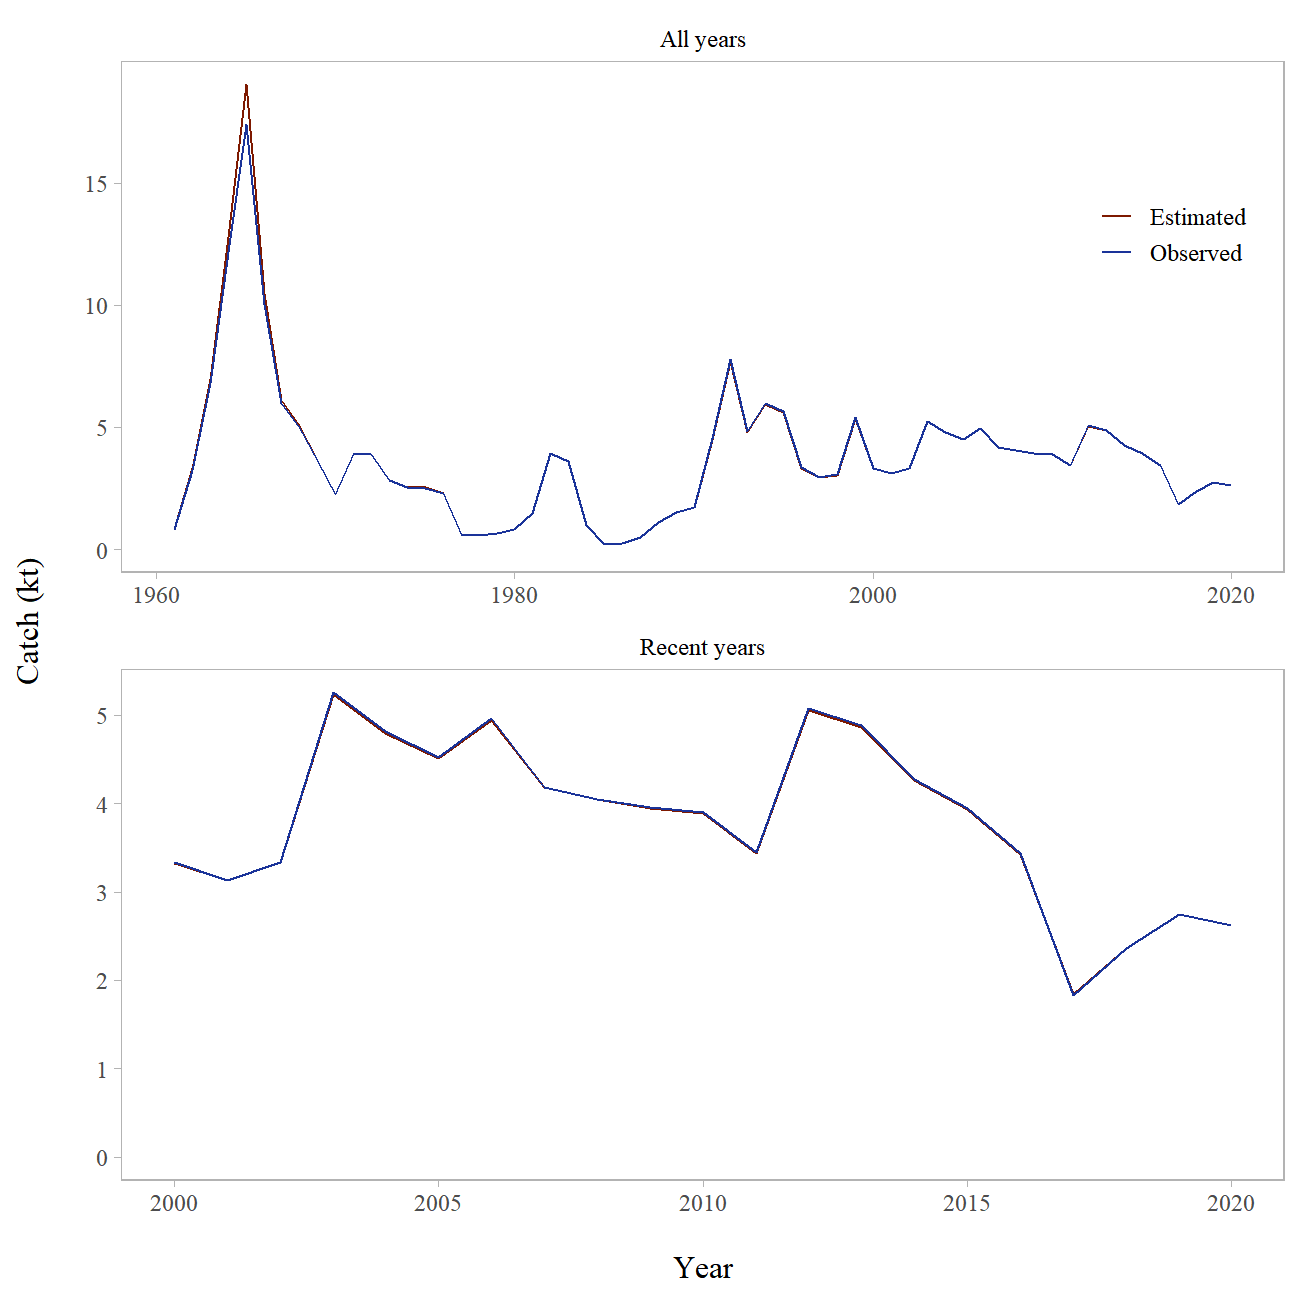
\includegraphics[width=18.06in]{C:/Users/Ben.Williams/Desktop/northern_rockfish/2020/m18.2b/figs/catch} \caption{Estimated and observed long-term and recent commercial catch of northern rockfish in the Gulf of Alaska.}\label{fig:fig1}
\end{figure}

\begin{figure}
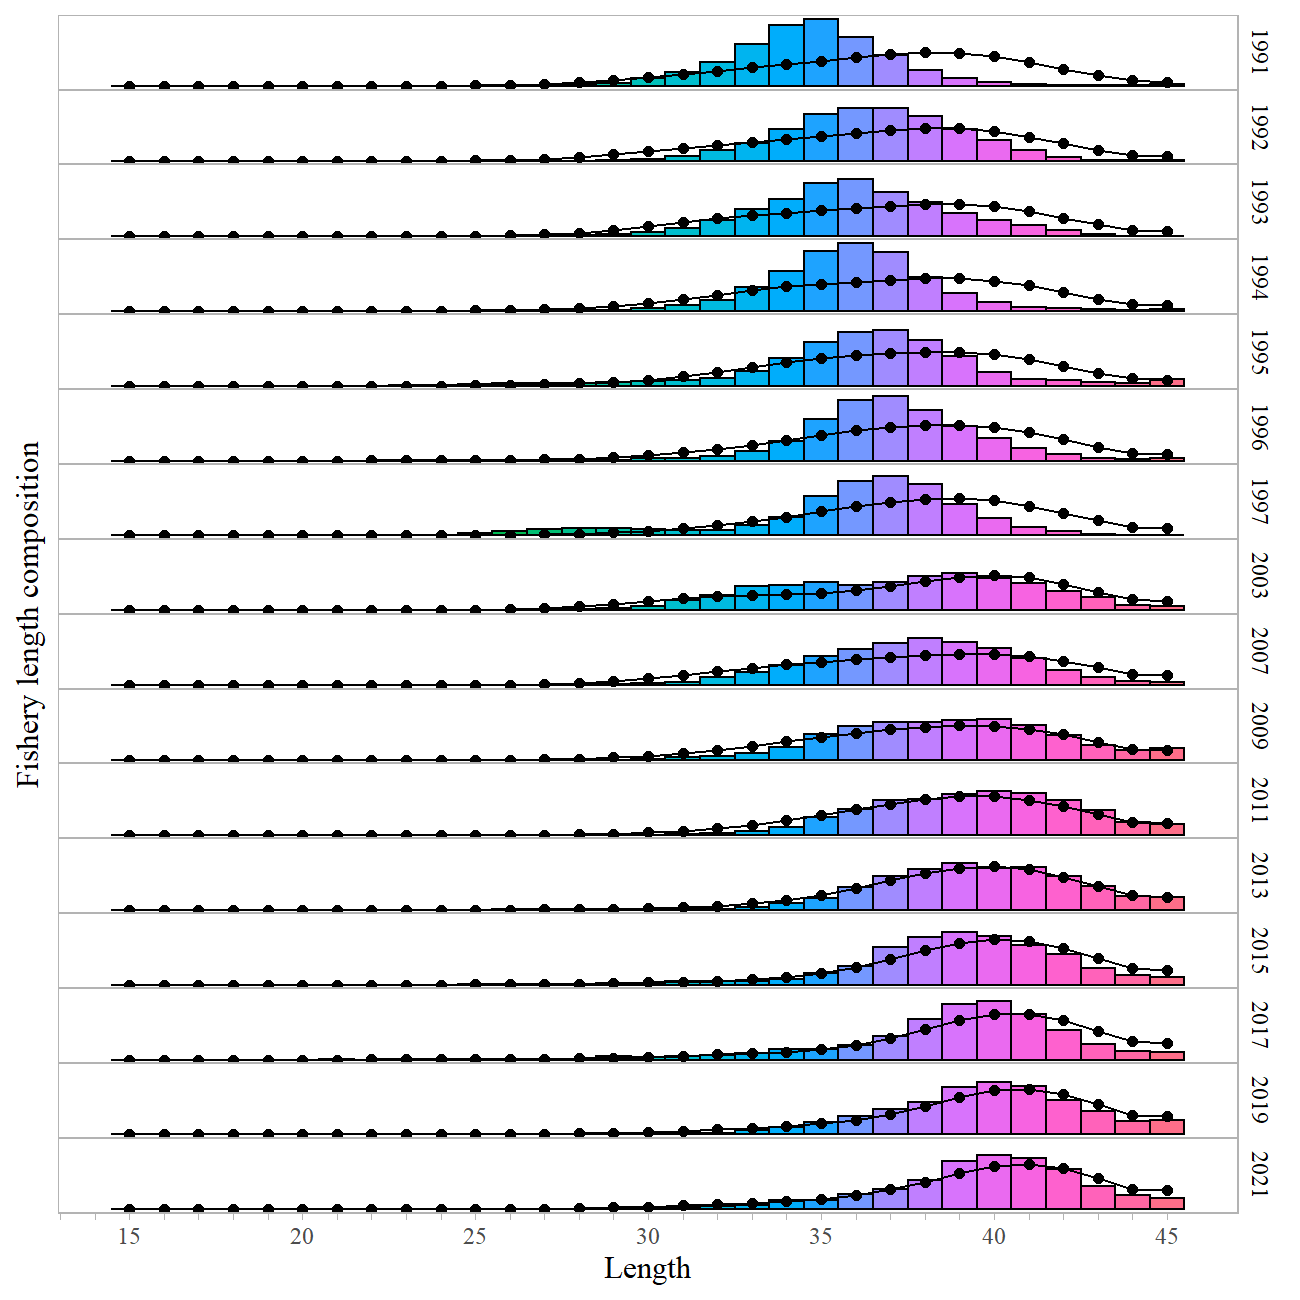
\includegraphics[width=18.06in]{C:/Users/Ben.Williams/Desktop/northern_rockfish/2020/m18.2b/figs/fishery_length_comp} \caption{Fishery length compositions for GOA northern rockfish. Observed = bars, lines are the predicted lengths from author recommended model.}\label{fig:fig2}
\end{figure}

\begin{figure}
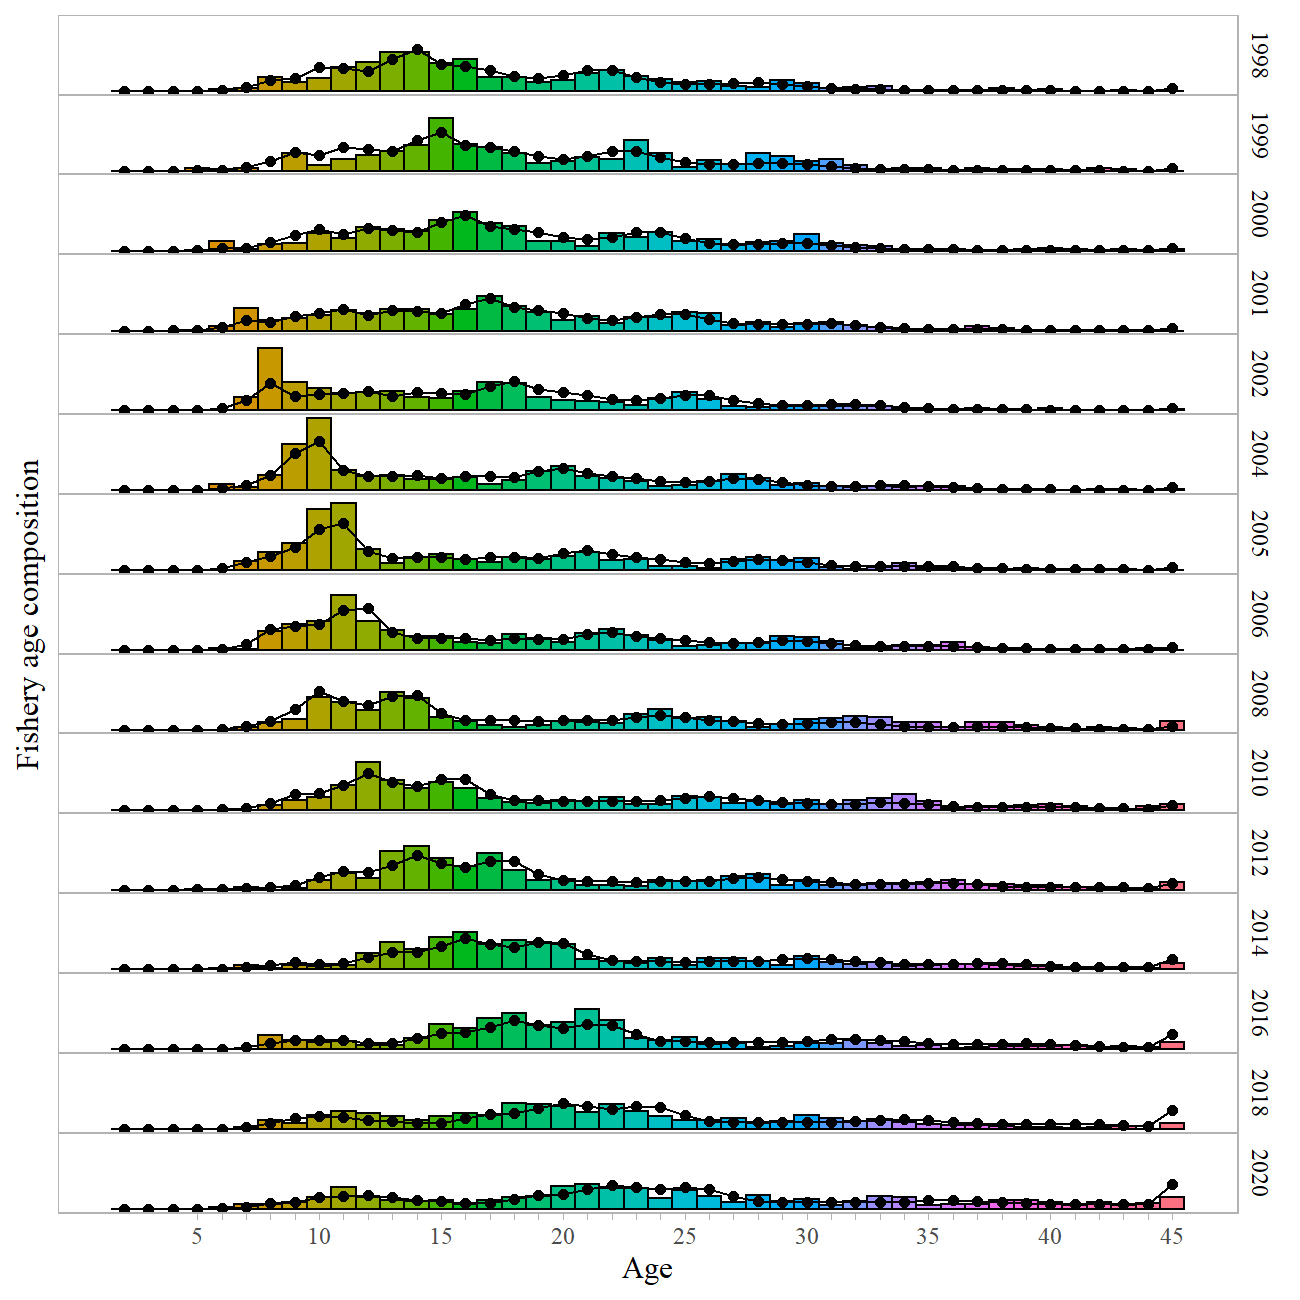
\includegraphics[width=18.06in]{C:/Users/Ben.Williams/Desktop/northern_rockfish/2020/m18.2b/figs/fishery_age_comp} \caption{Fishery age compositions for GOA northern rockfish. Observed = bars, lines are the predicted lengths from author recommended model.}\label{fig:fig3}
\end{figure}

\begin{figure}
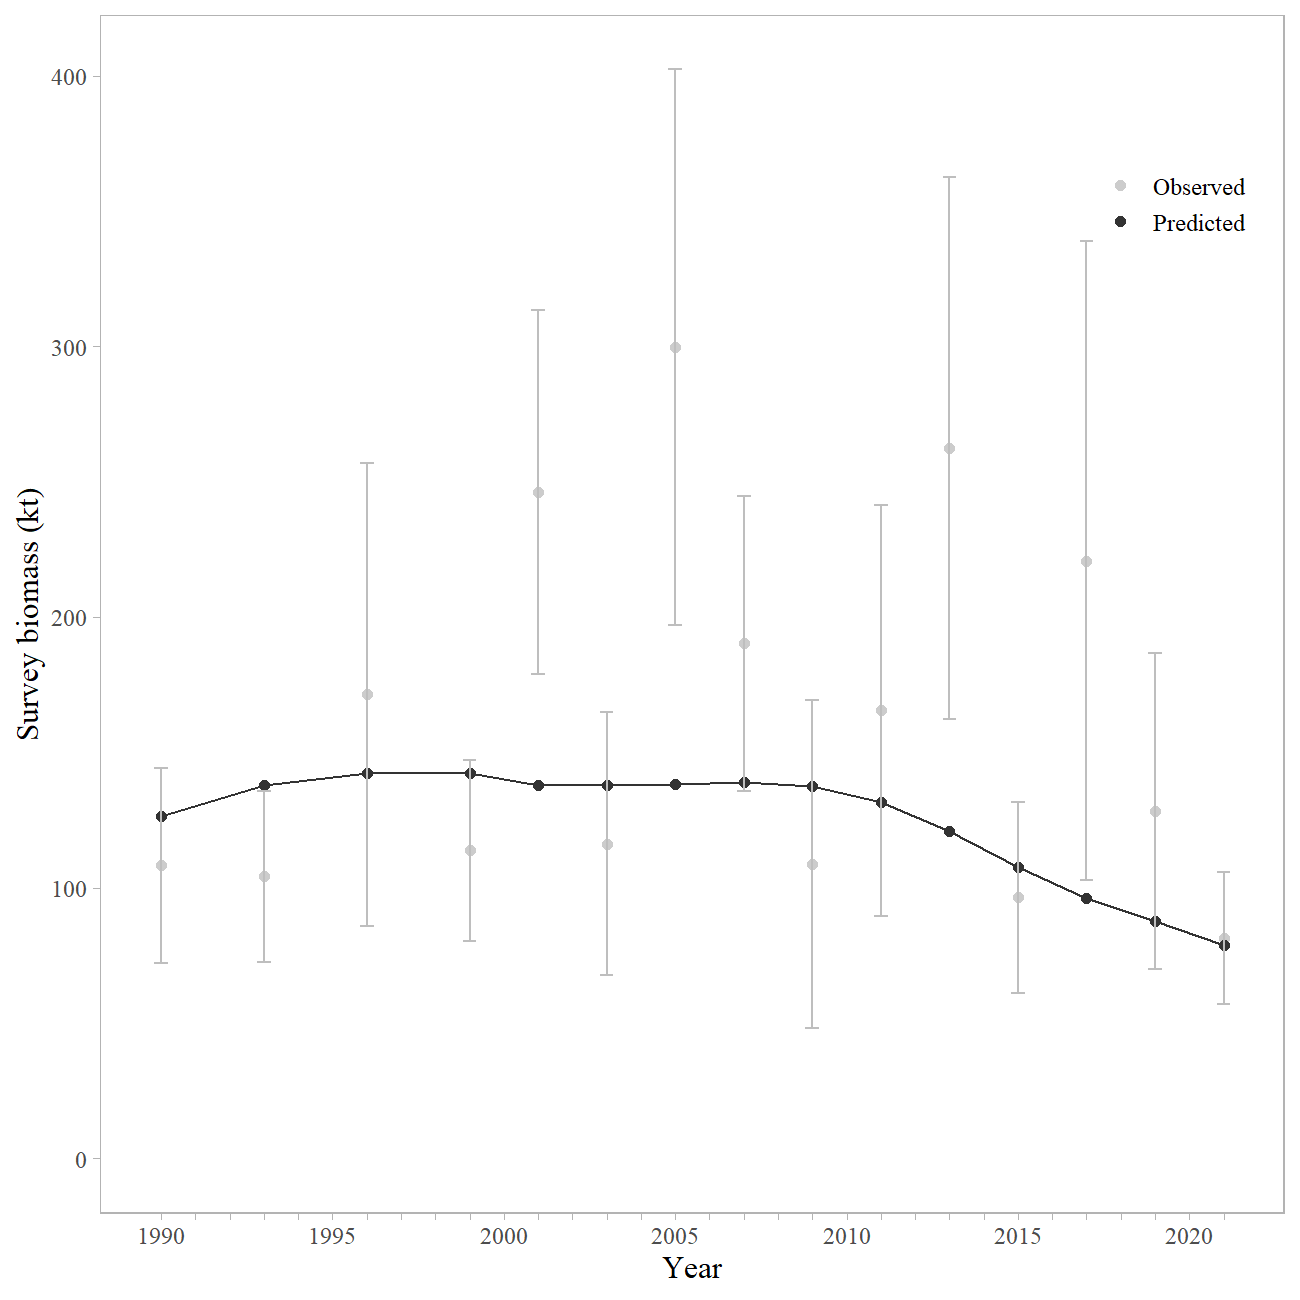
\includegraphics[width=18.06in]{C:/Users/Ben.Williams/Desktop/northern_rockfish/2020/m18.2b/figs/srv1_biomass} \caption{Observed and predicted GOA northern rockfish trawl survey VAST model-based index of biomass.}\label{fig:fig4}
\end{figure}

\begin{figure}
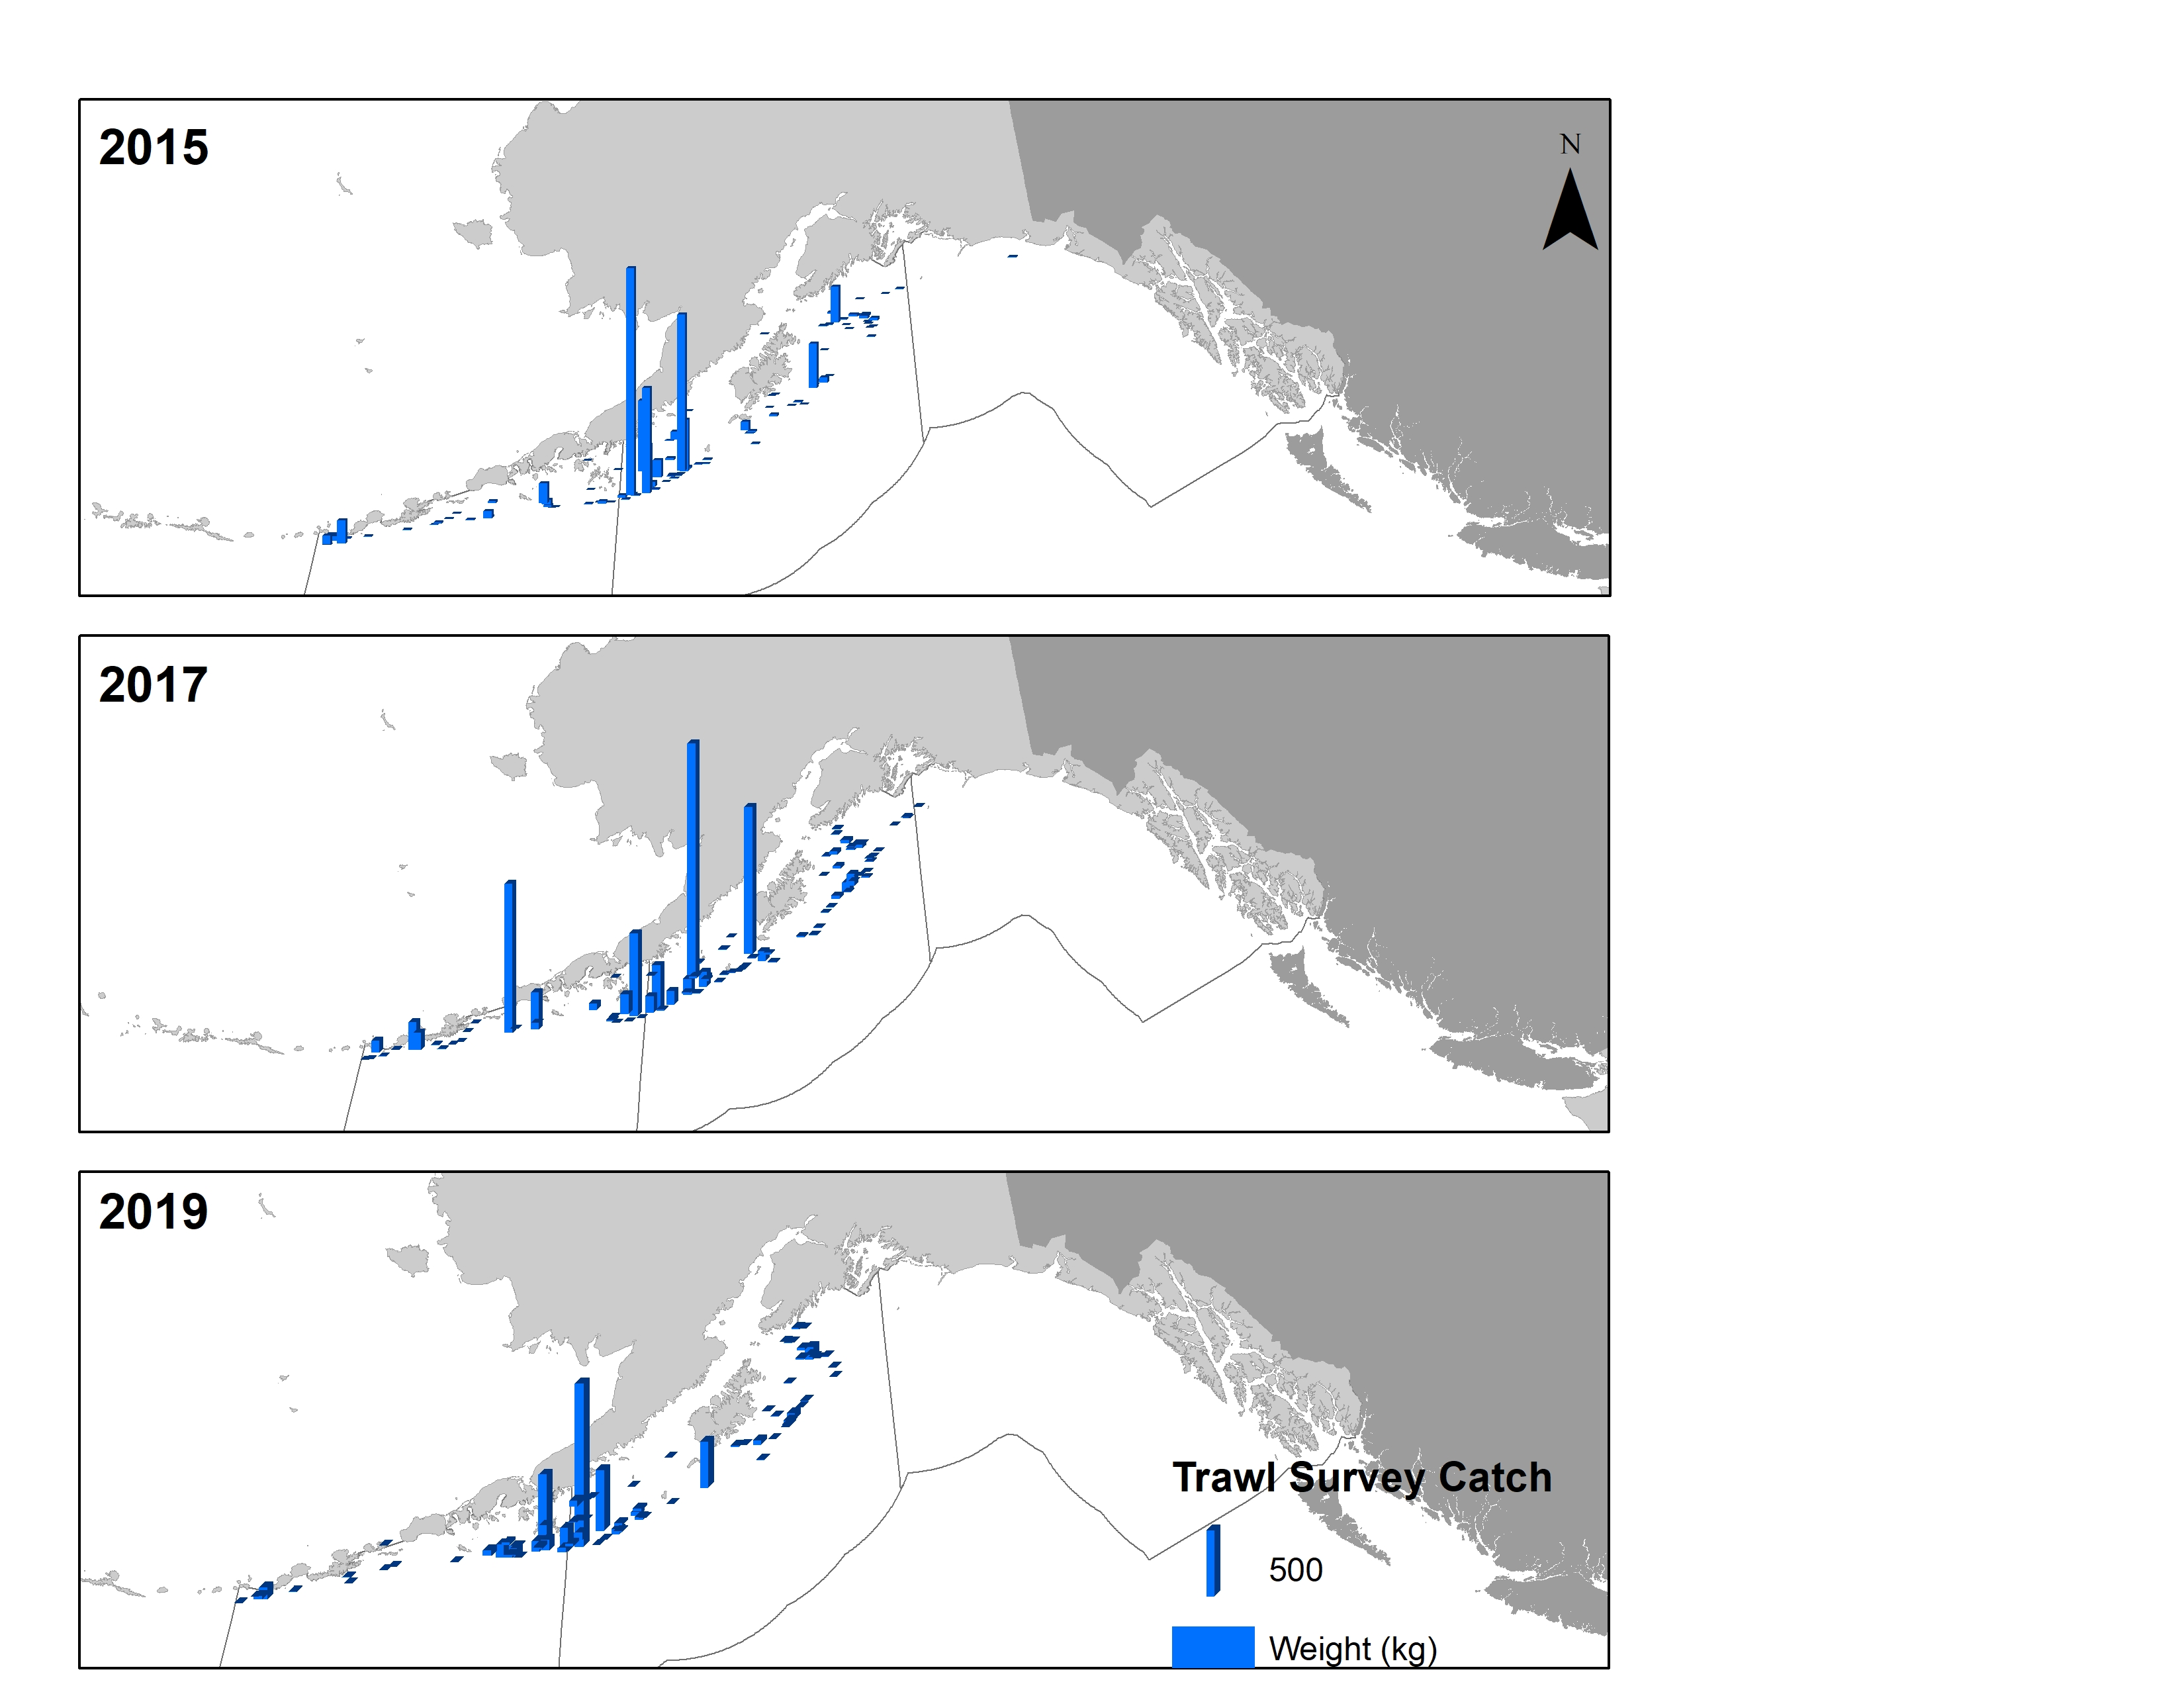
\includegraphics[width=45.83in]{C:/Users/Ben.Williams/Desktop/northern_rockfish/2020/m18.2b/figs/survey_catch} \caption{Spatial distribution of trawl survey catch for northern rockfish in the Gulf of Alaska .}\label{fig:fig5}
\end{figure}

\begin{figure}
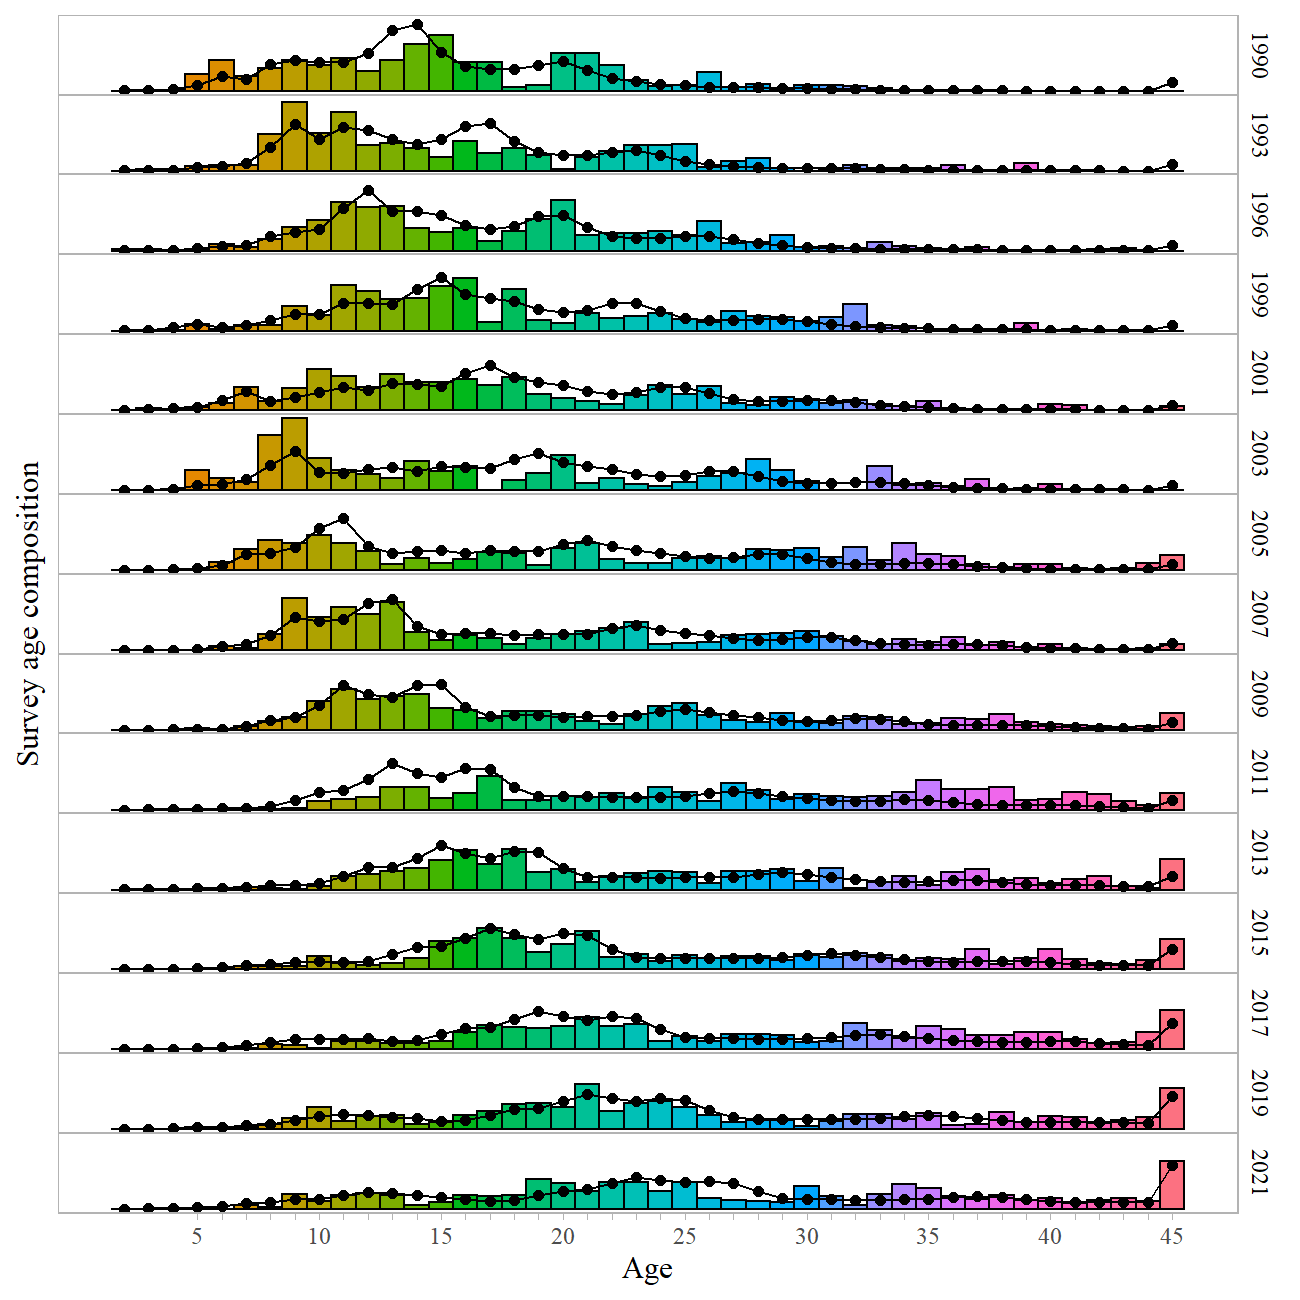
\includegraphics[width=18.06in]{C:/Users/Ben.Williams/Desktop/northern_rockfish/2020/m18.2b/figs/survey_age_comp} \caption{Trawl survey age composition by year for GOA northern rockfish. Observed = bars, predicted from author recommended model = line with circles.}\label{fig:fig6}
\end{figure}

\begin{figure}
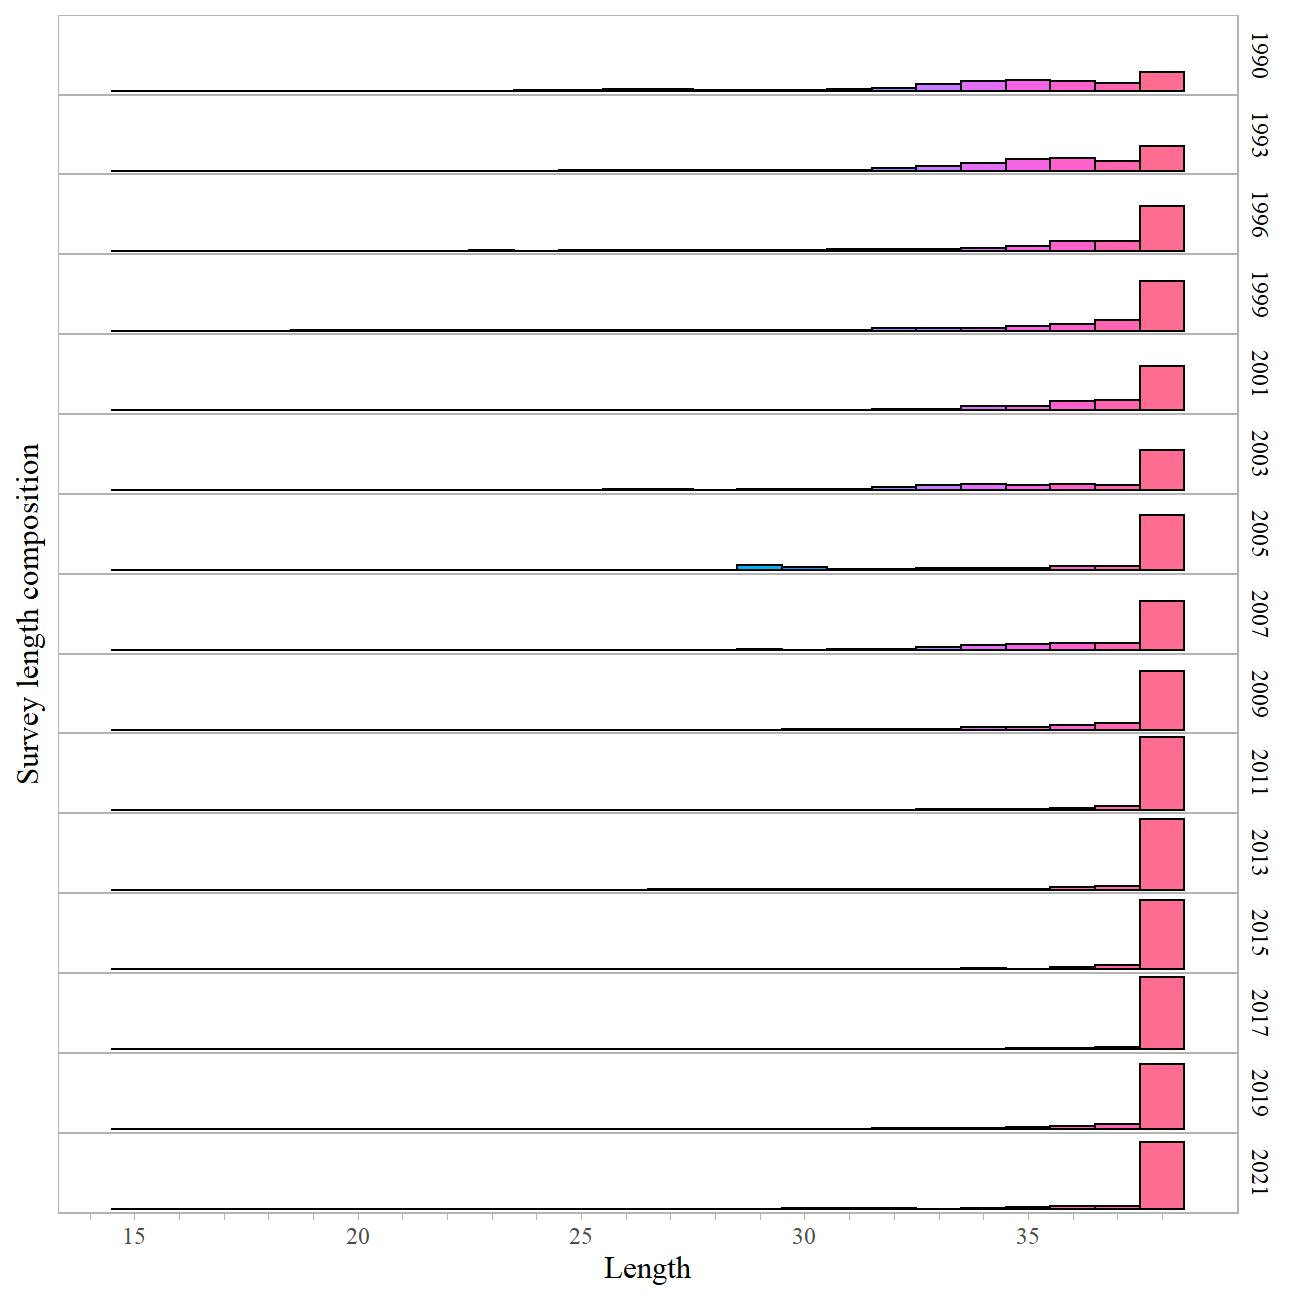
\includegraphics[width=18.06in]{C:/Users/Ben.Williams/Desktop/northern_rockfish/2020/m18.2b/figs/survey_length_comp} \caption{Trawl survey length composition by year for GOA northern rockfish. Survey length composition is not used in the model as age composition is available for these years.}\label{fig:fig7}
\end{figure}

\begin{figure}
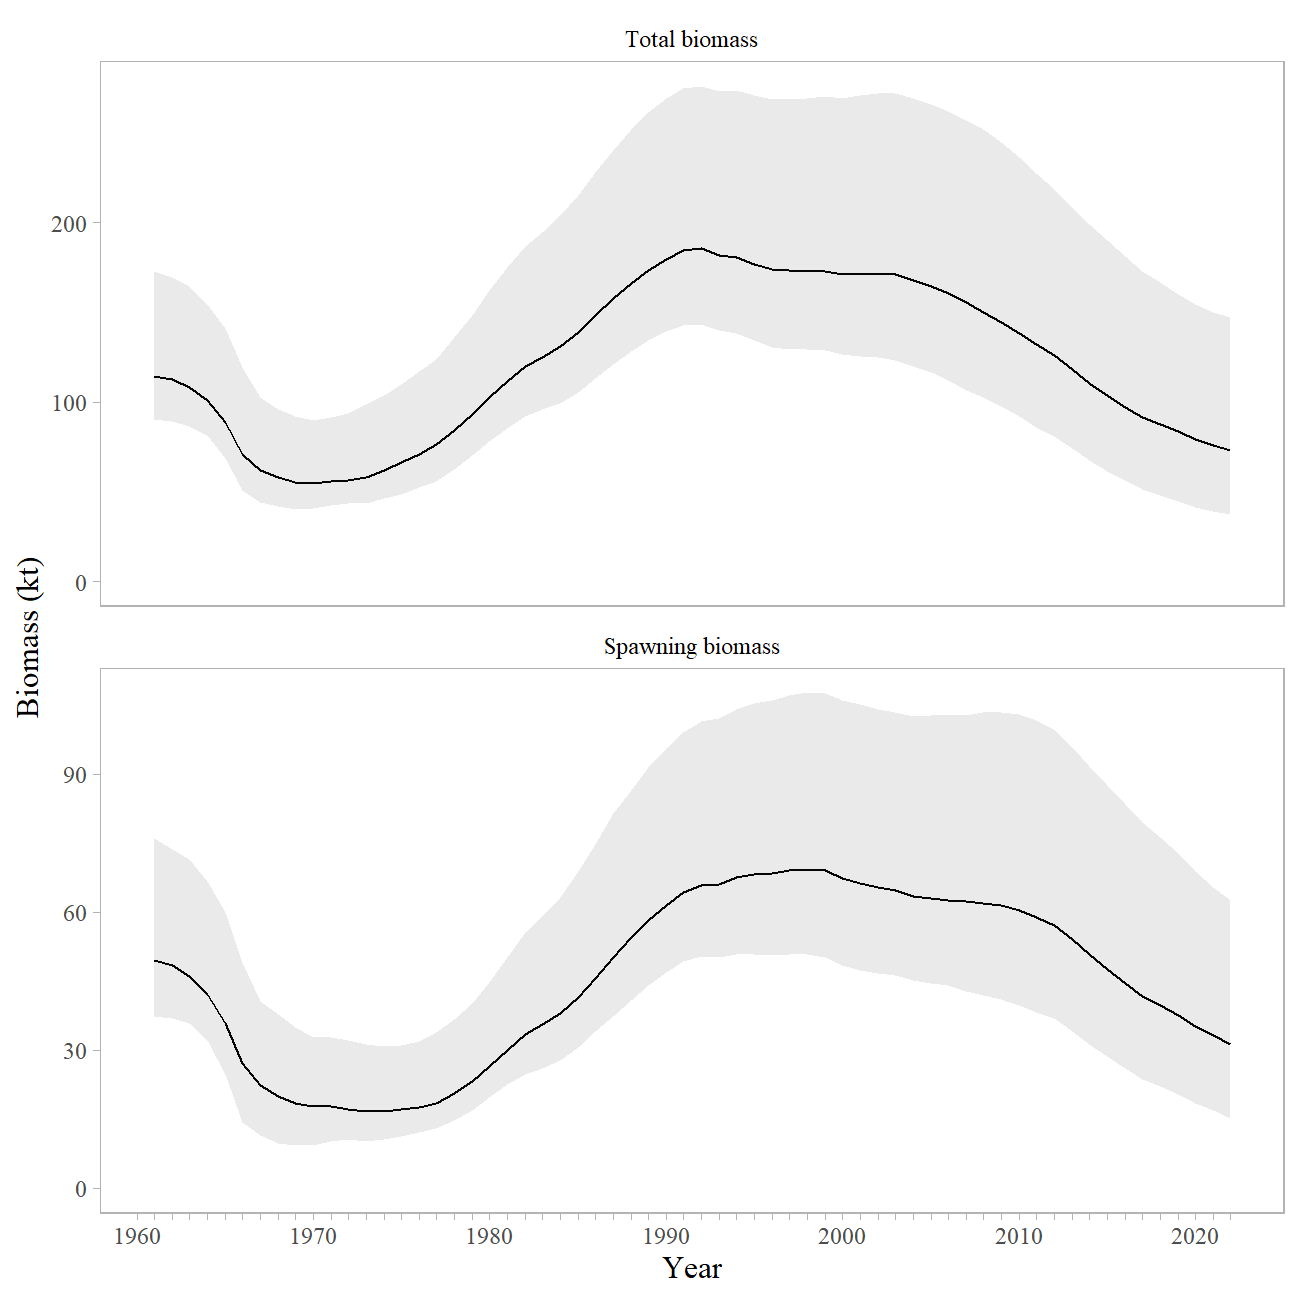
\includegraphics[width=18.06in]{C:/Users/Ben.Williams/Desktop/northern_rockfish/2020/m18.2b/figs/est_biomass} \caption{Model estimated total biomass and spawning biomass with 95\% credible intervals determined by MCMC (shaded) for Gulf of Alaska northern rockfish.}\label{fig:fig9}
\end{figure}

\begin{figure}
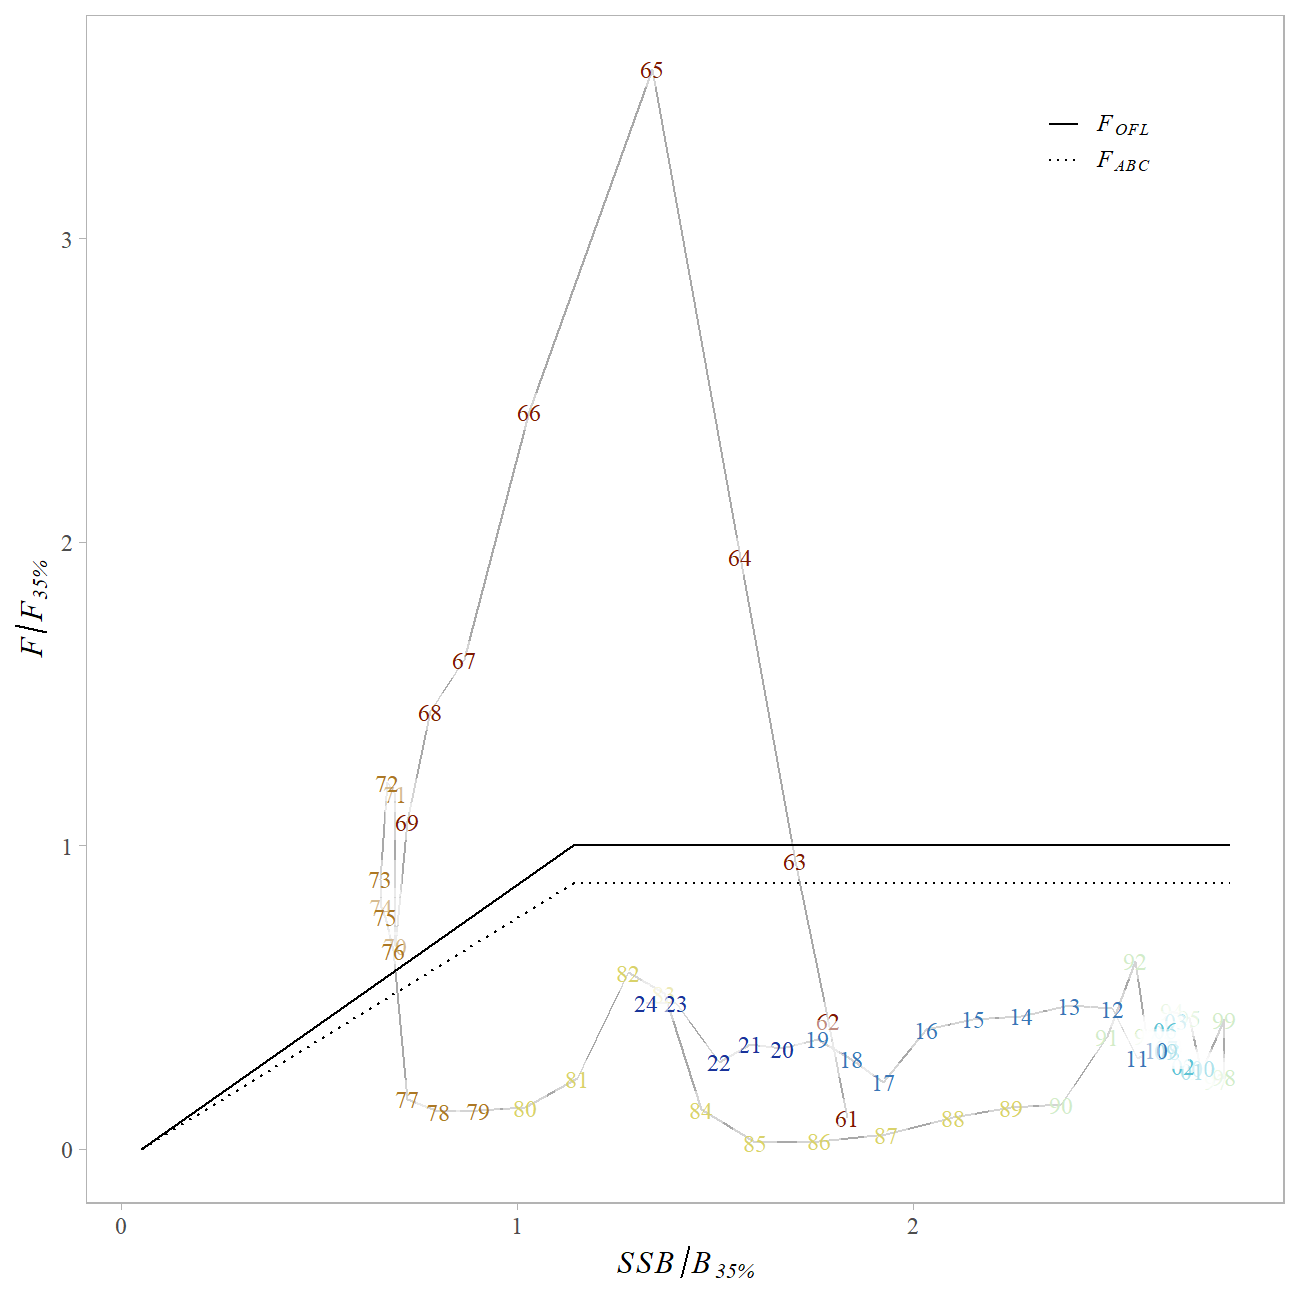
\includegraphics[width=18.06in]{C:/Users/Ben.Williams/Desktop/northern_rockfish/2020/m18.2b/figs/phase_plane} \caption{Time series of northern rockfish estimated spawning biomass (SSB) relative to $B_{35\%}$ and fishing mortality ($F$) relative to $F_{35\%}$ for author recommended model.}\label{fig:fig10}
\end{figure}

\begin{figure}
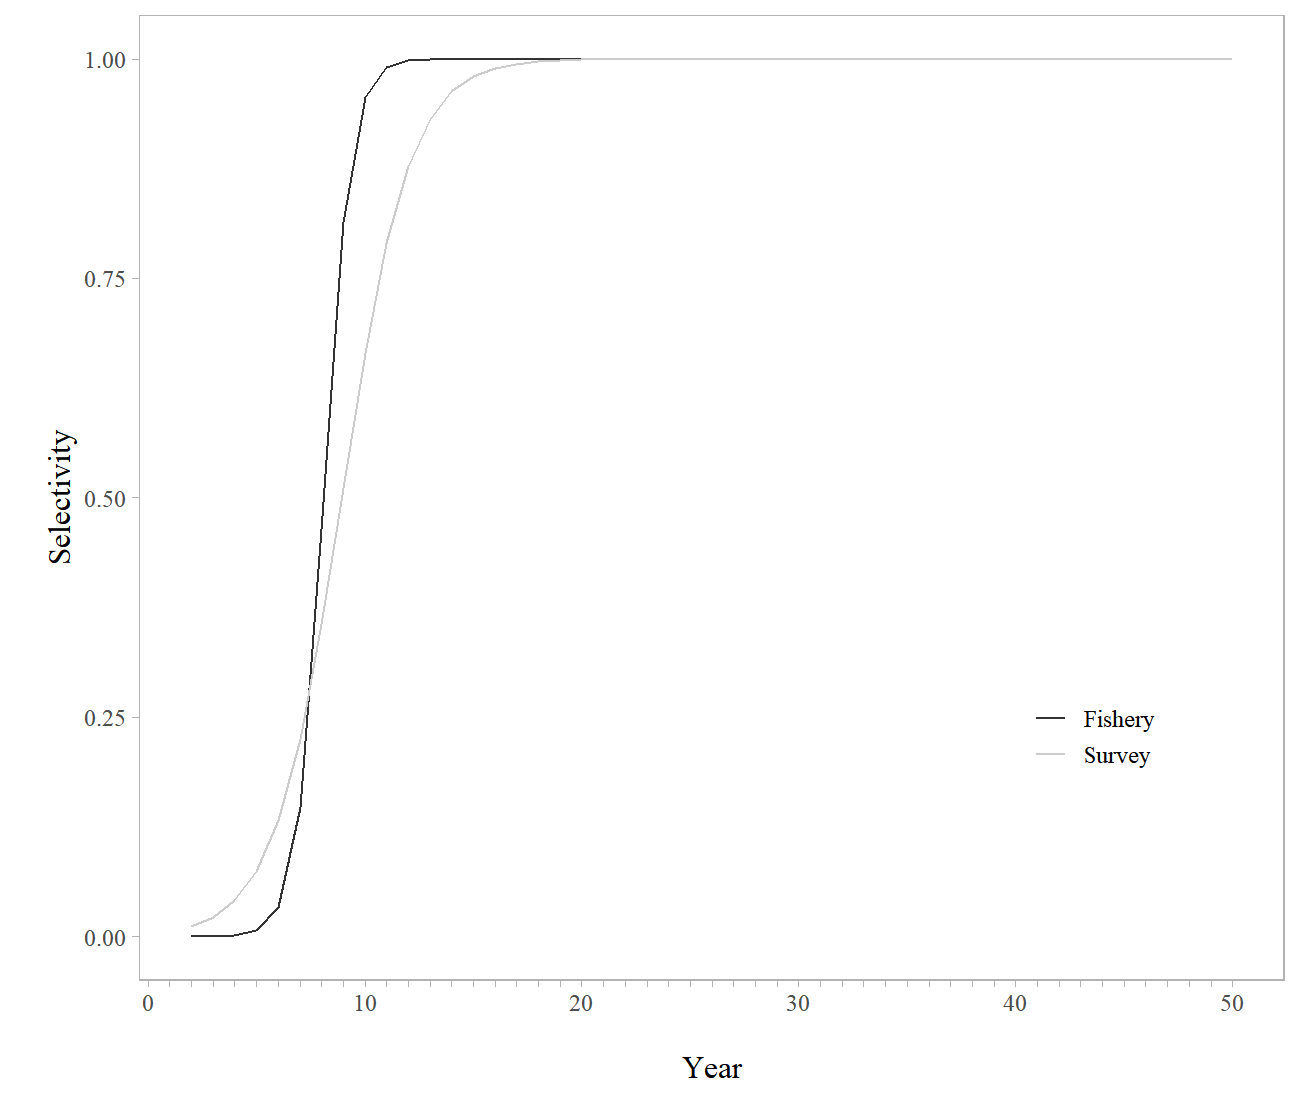
\includegraphics[width=18.06in]{C:/Users/Ben.Williams/Desktop/northern_rockfish/2020/m18.2b/figs/selex} \caption{Fishery and survey estimates of selectivity for GOA northern rockfish based on the authors recommended model.}\label{fig:fig11}
\end{figure}

\begin{figure}
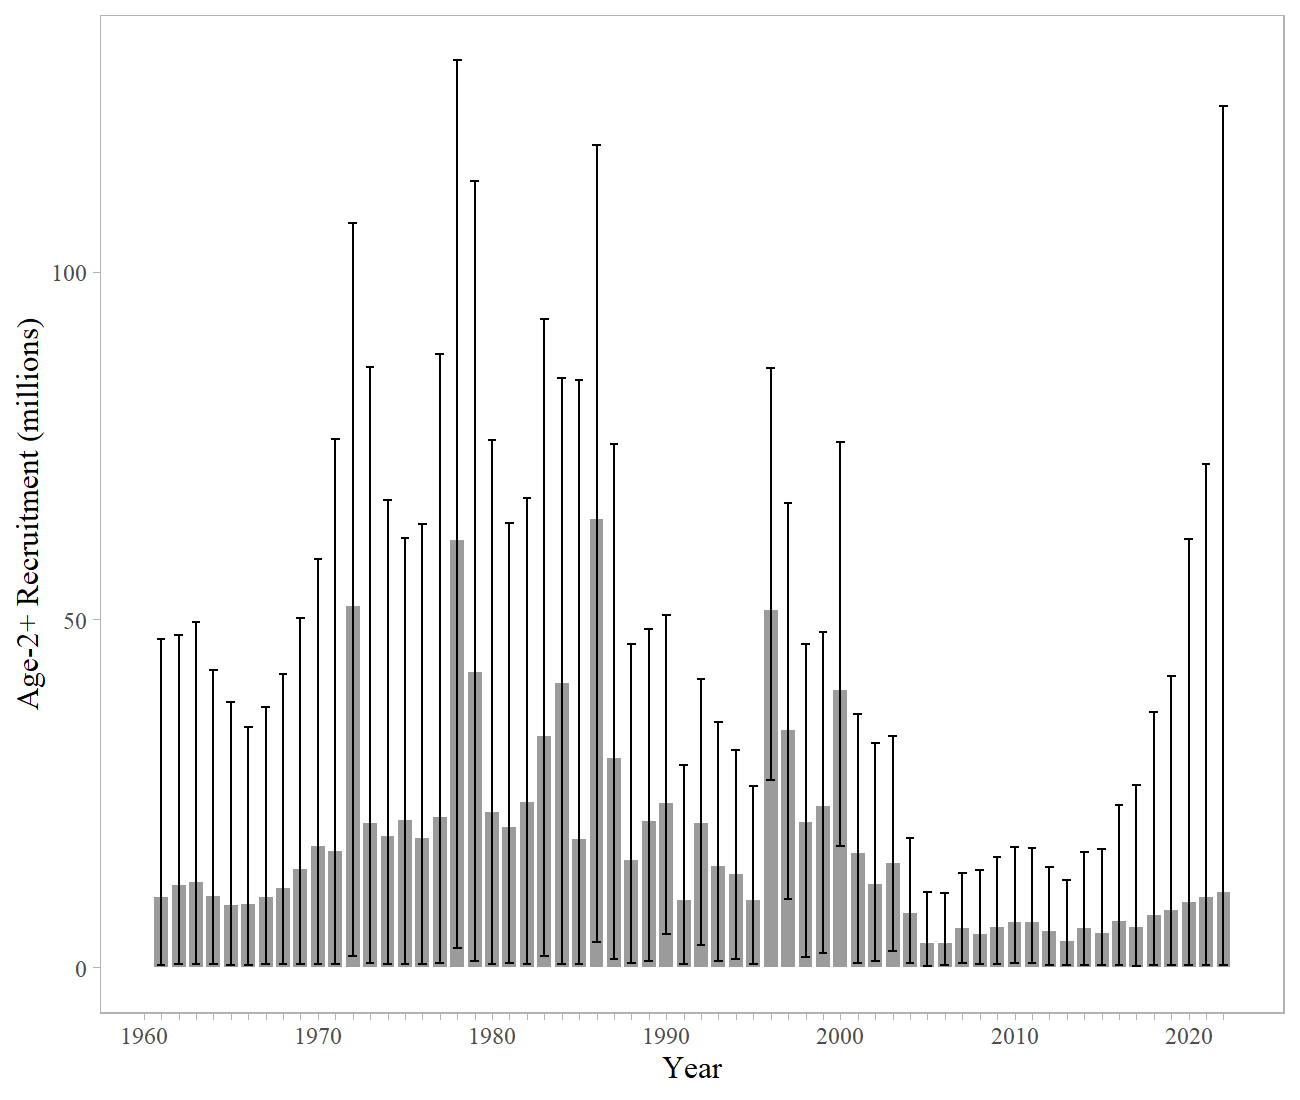
\includegraphics[width=18.06in]{C:/Users/Ben.Williams/Desktop/northern_rockfish/2020/m18.2b/figs/recruits} \caption{Estimates of age-2 recruitment with 95\% credible intervals for GOA northern rockfish.}\label{fig:fig12}
\end{figure}

\begin{figure}
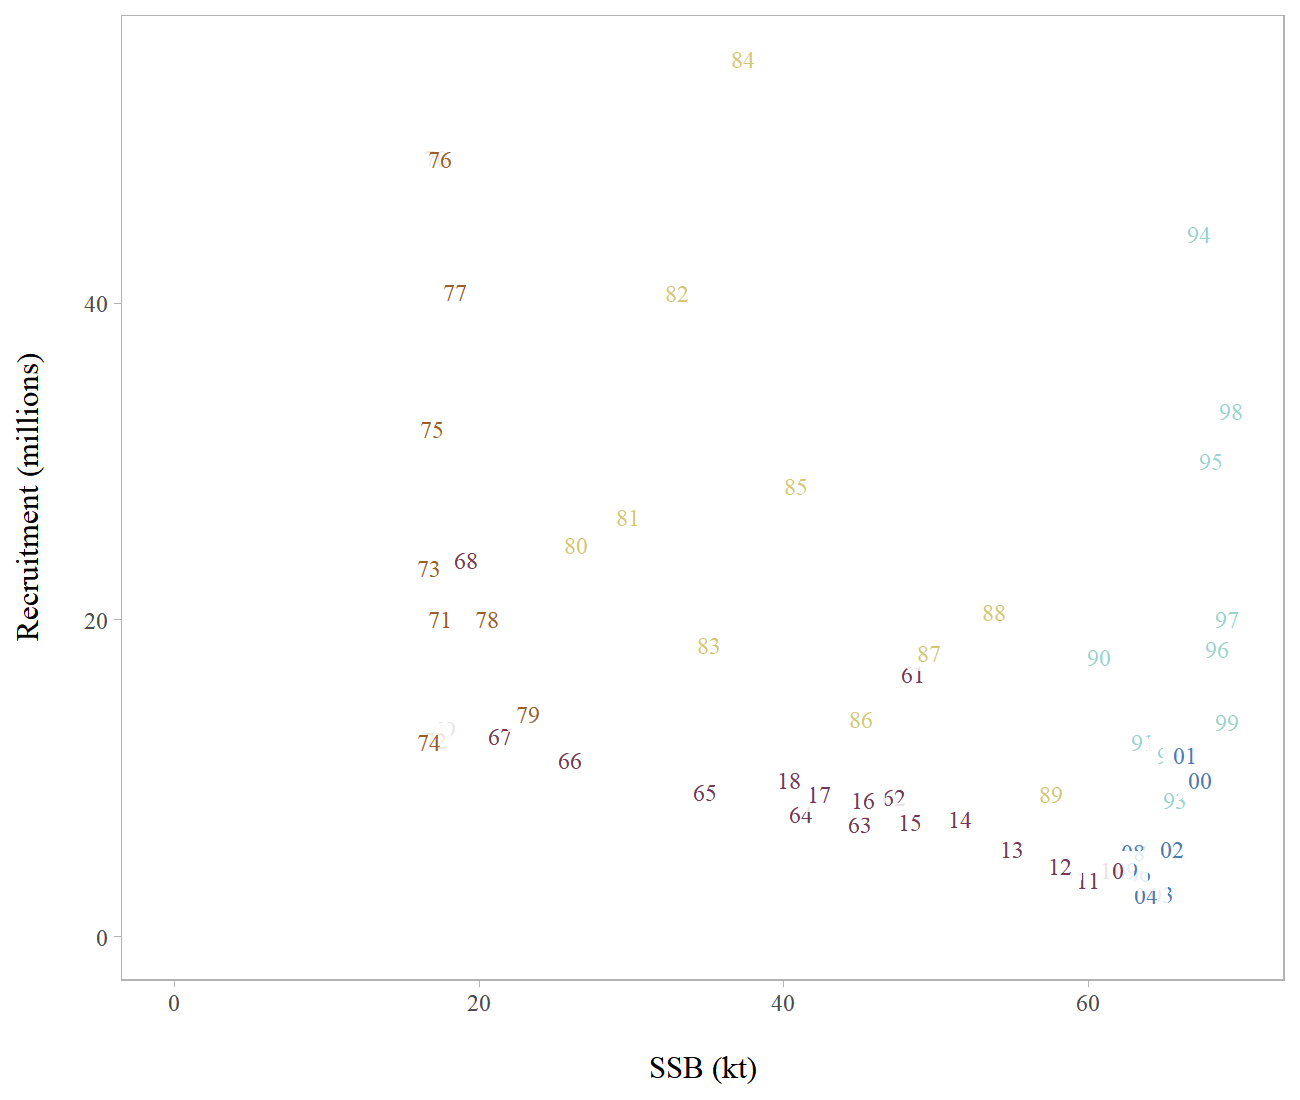
\includegraphics[width=18.06in]{C:/Users/Ben.Williams/Desktop/northern_rockfish/2020/m18.2b/figs/recr-ssb} \caption{Female spawning stock biomass (SSB) and recruitment (by year class) for GOA northern rockfish.}\label{fig:fig13}
\end{figure}

\begin{figure}
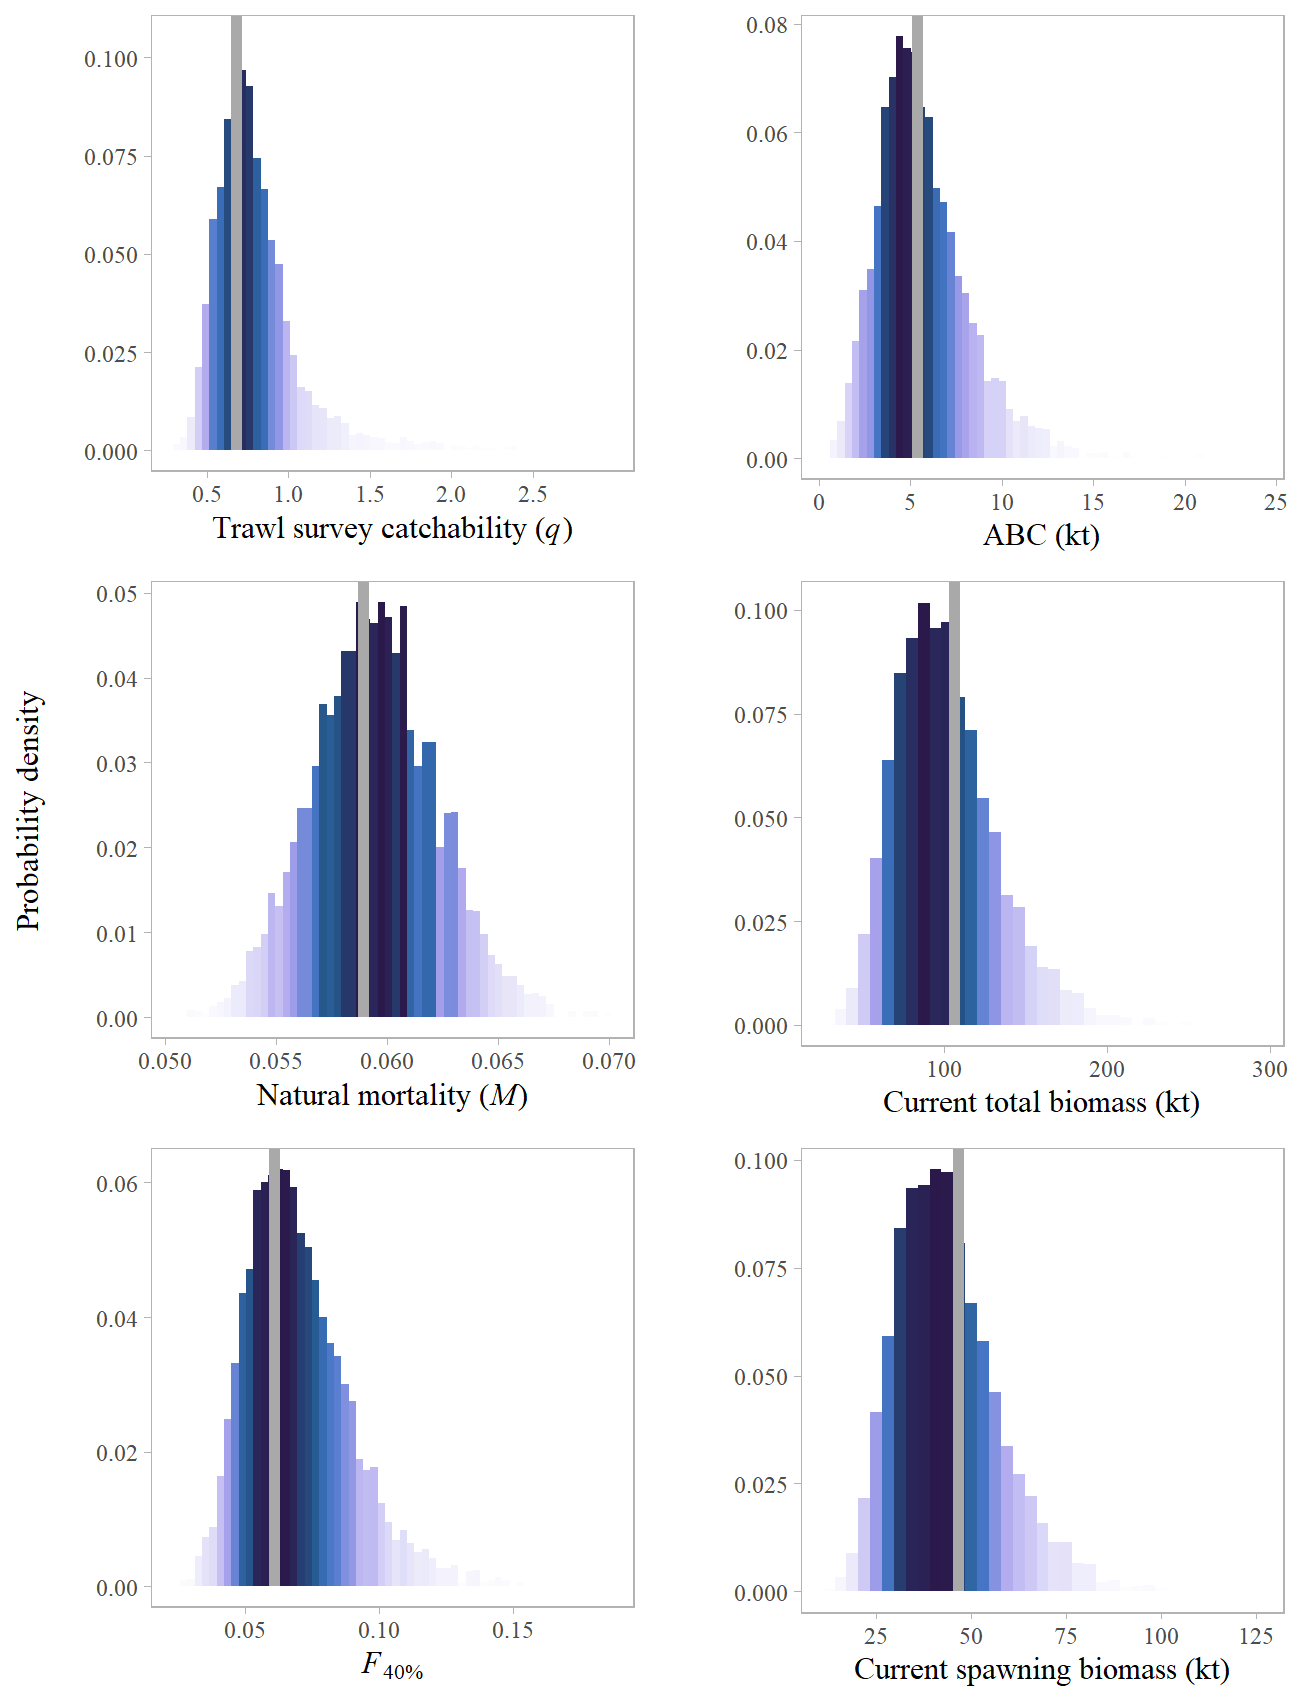
\includegraphics[width=18.06in]{C:/Users/Ben.Williams/Desktop/northern_rockfish/2020/m18.2b/figs/hists} \caption{Histograms of estimated posterior distributions for key parameters derived from the MCMC for GOA northern rockfish. Vertical lines represent the maximum likelihood estimate for comparison with the MCMC results.}\label{fig:fig14}
\end{figure}

\begin{figure}
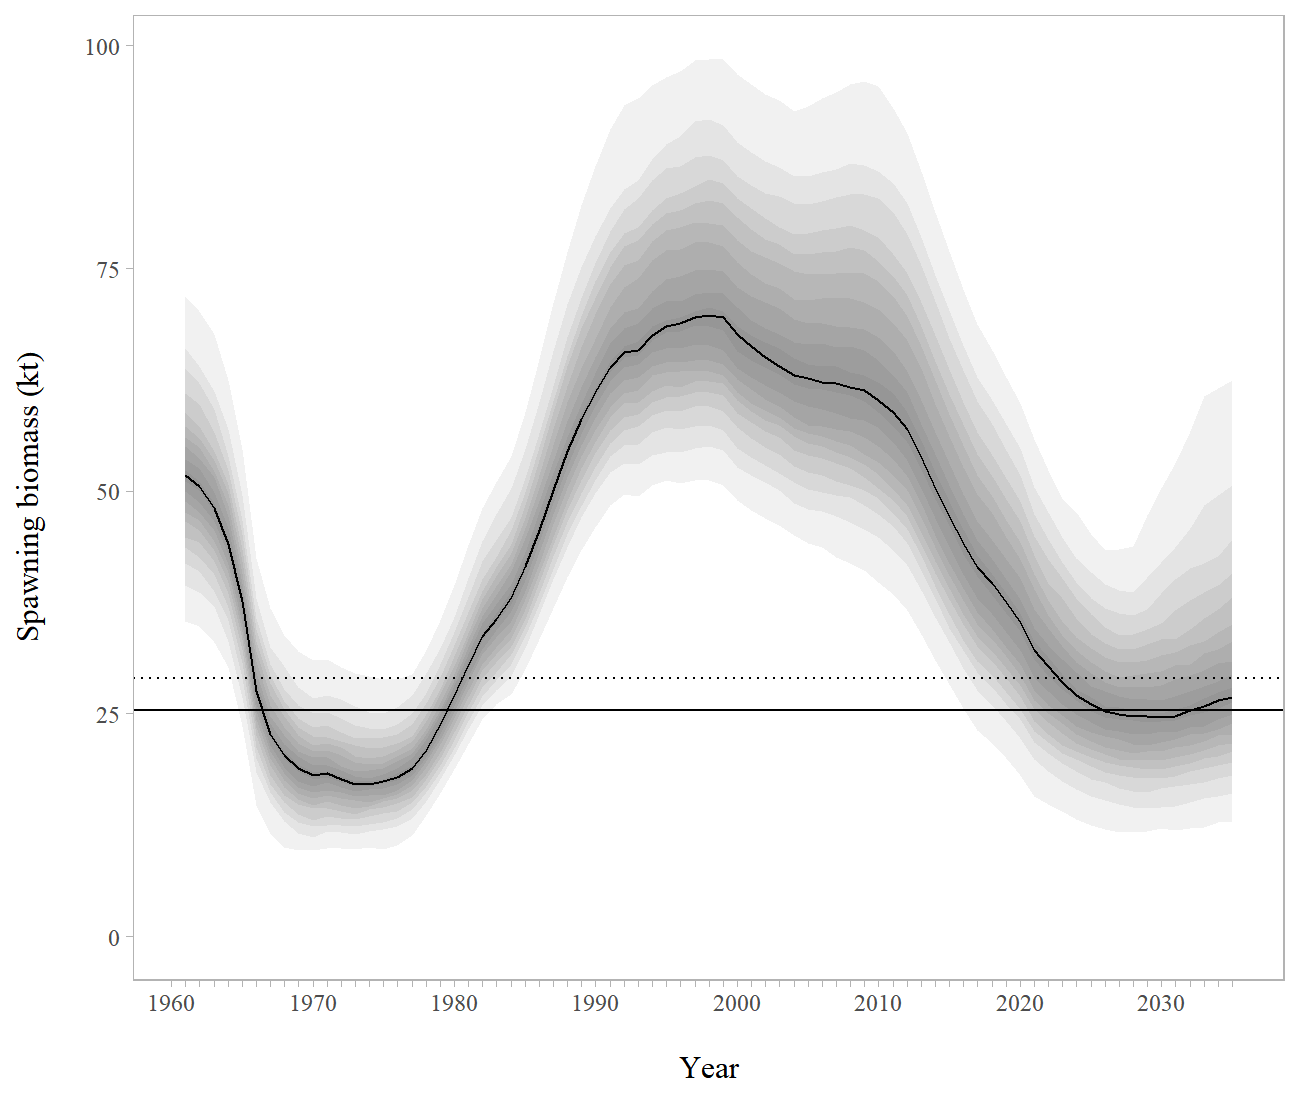
\includegraphics[width=18.06in]{C:/Users/Ben.Williams/Desktop/northern_rockfish/2020/m18.2b/figs/swath} \caption{Median spawning stock biomass from MCMC simulations with Bayesian credible intervals including projections through 2035 , when managing under Scenario 2. Assumes the same average yield ratio forward in time. Dotted horizontal line is $B_{40\%}$ and solid horizontal line is $B_{35\%}$ based on recruitments from 1977-2018. Each shade is 5\% of the posterior distribution.}\label{fig:fig15}
\end{figure}

\begin{figure}
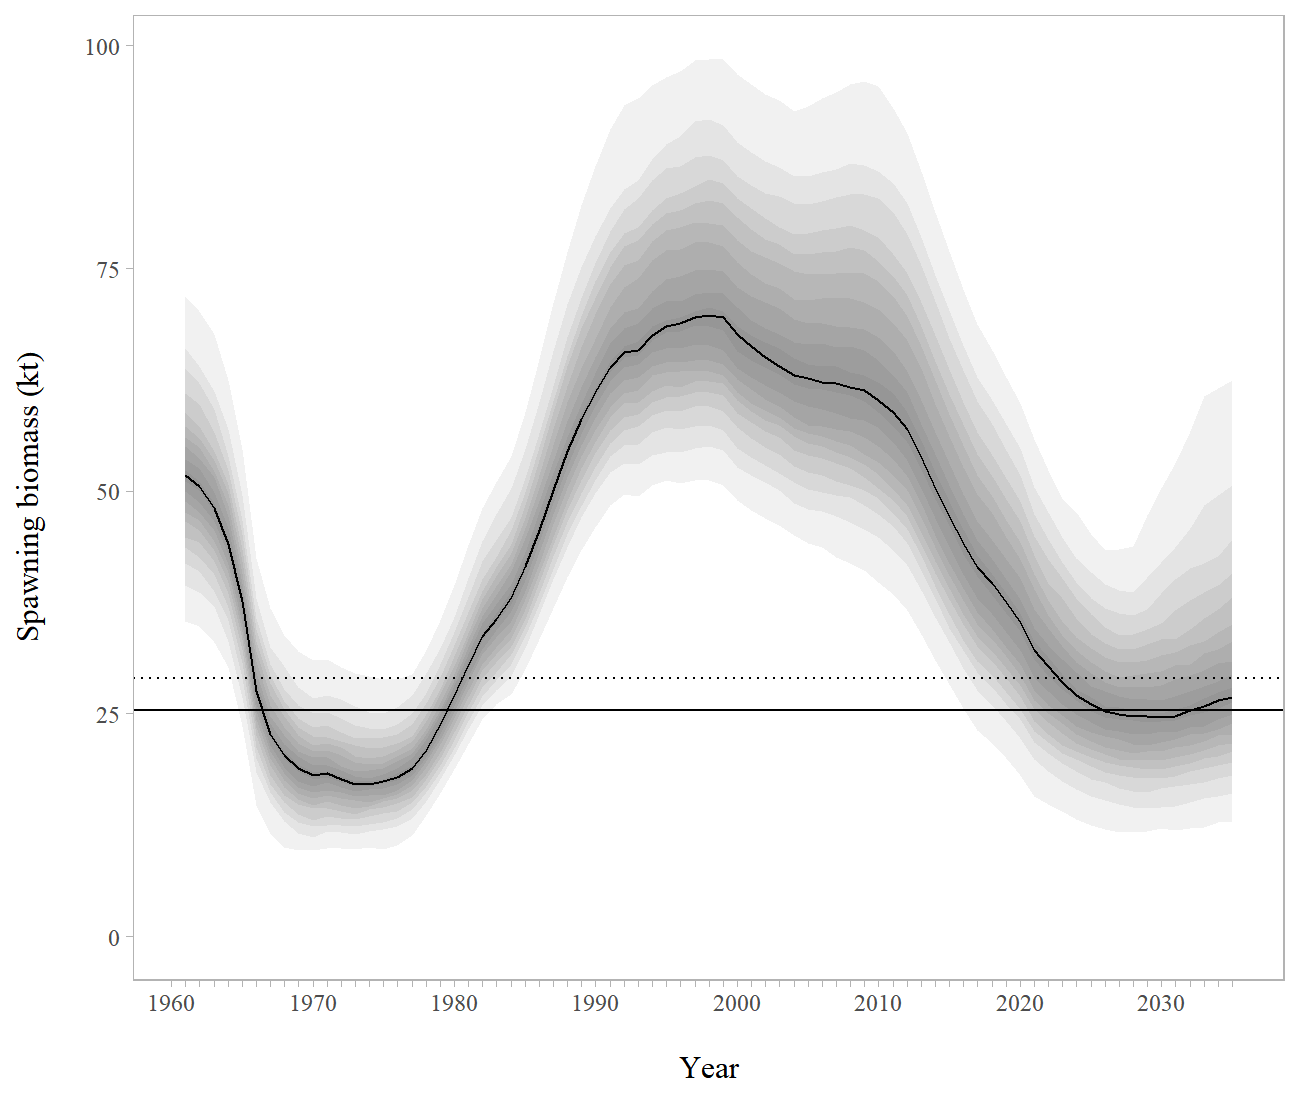
\includegraphics[width=18.06in]{C:/Users/Ben.Williams/Desktop/northern_rockfish/2020/m18.2b/figs/swath} \caption{Retrospective peels of estimated female spawning biomass for the past 10 years from the author recommended model and the percent difference in female spawning biomass from the recommended model in the terminal year. Shaded areas are Bayesian 95\% credible intervals derived from MCMC.}\label{fig:fig16}
\end{figure}

\pagebreak

\end{document}
